\section{Domänenmodellierung}

\begin{concept}{Domänenmodell}\\
Ein Domänenmodell ist ein vereinfachtes UML-Klassendiagramm zur Darstellung der Fachdomäne:
\begin{itemize}
    \item Konzepte als Klassen
    \item Eigenschaften als Attribute (ohne Typangabe)
    \item Beziehungen als Assoziationen mit Multiplizitäten
    \item Optional: Aggregationen/Kompositionen
\end{itemize}
\end{concept}

\begin{KR}{Domänenmodell Erstellung}\\
\textbf{Schritt 1: Konzepte identifizieren}
\begin{itemize}
    \item Substantive aus Anforderungen extrahieren
    \item Kategorien prüfen:
    \begin{itemize}
        \item Physische Objekte
        \item Kataloge
        \item Container
        \item Externe Systeme
        \item Rollen von Personen
        \item Artefakte (Pläne, Dokumente)
        \item Zahlungsinstrumente
    \end{itemize}
    \item \textbf{Wichtig:} Keine Softwareklassen modellieren!
\end{itemize}

\textbf{Schritt 2: Attribute definieren}
\begin{itemize}
    \item Nur wichtige/einfache Attribute
    \item Typische Kategorien:
    \begin{itemize}
        \item Transaktionsdaten
        \item Teil-Ganzes Beziehungen
        \item Beschreibungen
        \item Verwendungszwecke
    \end{itemize}
    \item \textbf{Wichtig:} Beziehungen als Assoziationen, nicht als Attribute!
\end{itemize}

\textbf{Schritt 3: Beziehungen modellieren}
\begin{itemize}
    \item Assoziationen zwischen Konzepten identifizieren
    \item Multiplizitäten festlegen
    \item Art der Beziehung bestimmen
    \item Richtung der Assoziation falls nötig
\end{itemize}
\end{KR}

\subsubsection{Analysemuster im Domänenmodell}
Bewährte Strukturen für wiederkehrende Modellierungssituationen:

\begin{concept}{1. Beschreibungsklassen}
\begin{itemize}
    \item Trennung von Instanz und Beschreibung
    \item Beispiel: Artikel vs. Artikelbeschreibung
    \item Vermeidet Redundanz bei gleichen Eigenschaften
\end{itemize}
\end{concept}

\begin{concept}{2. Generalisierung/Spezialisierung}
\begin{itemize}
    \item 100\% Regel: Alle Instanzen der Spezialisierung sind auch Instanzen der Generalisierung
    \item "IS-A" Beziehung
    \item Gemeinsame Attribute/Assoziationen als Grund für Generalisierung
\end{itemize}
\end{concept}

\begin{concept}{3. Komposition}
\begin{itemize}
    \item Starke Teil-Ganzes Beziehung
    \item Existenzabhängigkeit der Teile
\end{itemize}
\end{concept}

\begin{concept}{4. Zustandsmodellierung}
\begin{itemize}
    \item Zustände als eigene Hierarchie
    \item Vermeidet problematische Vererbung
\end{itemize}
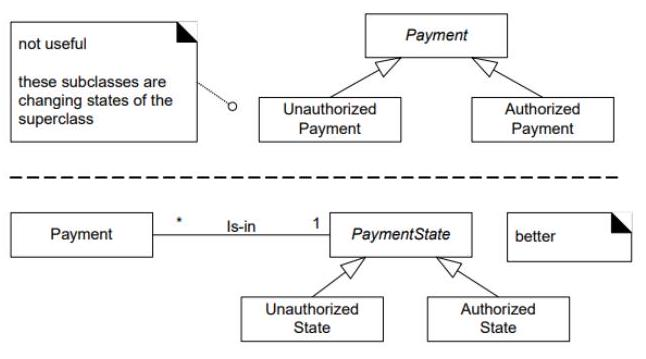
\includegraphics[width=0.9\linewidth]{images/2024_12_29_0d1d7b5551ea1b4b41bdg-07(1)}
\end{concept}

\begin{concept}{5. Rollen}
\begin{itemize}
    \item Unterschiedliche Rollen eines Konzepts
    \item Als eigene Konzepte oder Assoziationen
\end{itemize}
\end{concept}

\begin{concept}{6. Assoziationsklassen}
\begin{itemize}
    \item Attribute einer Beziehung
    \item Eigene Klasse für die Assoziation
\end{itemize}
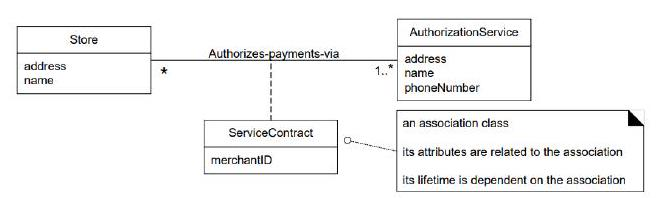
\includegraphics[width=\linewidth]{images/2024_12_29_0d1d7b5551ea1b4b41bdg-07}
\end{concept}

\begin{concept}{7. Wertobjekte}
\begin{itemize}
    \item Masseinheiten als eigene Konzepte
    \item Zeitintervalle als Konzepte
    \item Vermeidet primitive Obsession
\end{itemize}
\end{concept}

\begin{example}{Domänenmodell Online-Shop}
\textbf{Aufgabe:} Erstellen Sie ein Domänenmodell für einen Online-Shop mit Warenkorb-Funktion.

\textbf{Lösung:}
\begin{itemize}
    \item \textbf{Konzepte identifizieren:}
    \begin{itemize}
        \item Artikel (physisches Objekt)
        \item Artikelbeschreibung (Beschreibungsklasse)
        \item Warenkorb (Container)
        \item Bestellung (Transaktion)
        \item Kunde (Rolle)
    \end{itemize}
    \item \textbf{Attribute:}
    \begin{itemize}
        \item Artikelbeschreibung: name, preis, beschreibung
        \item Bestellung: datum, status
        \item Kunde: name, adresse
    \end{itemize}
    \item \textbf{Beziehungen:}
    \begin{itemize}
        \item Warenkorb gehört zu genau einem Kunde (Komposition)
        \item Warenkorb enthält beliebig viele Artikel
        \item Bestellung wird aus Warenkorb erstellt
    \end{itemize}
\end{itemize}
\end{example}

\begin{KR}{Typische Modellierungsfehler vermeiden}
\begin{itemize}
    \item \textbf{Keine Softwareklassen modellieren}
    \begin{itemize}
        \item Manager-Klassen vermeiden
        \item Keine technischen Helper-Klassen
    \end{itemize}
    
    \item \textbf{Keine Operationen modellieren}
    \begin{itemize}
        \item Fokus auf Struktur, nicht Verhalten
        \item Keine CRUD-Operationen
    \end{itemize}
    
    \item \textbf{Richtige Abstraktionsebene wählen}
    \begin{itemize}
        \item Nicht zu detailliert
        \item Nicht zu abstrakt
        \item Fachliche Begriffe verwenden
    \end{itemize}
    
    \item \textbf{Assoziationen statt Attribute}
    \begin{itemize}
        \item Beziehungen als Assoziationen modellieren
        \item Keine Objekt-IDs als Attribute
    \end{itemize}
\end{itemize}
\end{KR}